% Part 8 – Discussion, Limitations and Conclusions

% ---------------------------------------------------------------------------
% The final part of this report synthesises the theoretical insights and
% empirical findings from the preceding sections.  We provide a comparative
% discussion of energy–based models (EBMs) and noise–conditional score
% networks (NCSNs), analyse their strengths and weaknesses, highlight
% hyperparameter sensitivities, and outline the limitations of our
% implementations.  We conclude with reflections on future directions and
% ethical considerations.

\section{Discussion, Limitations and Conclusions}

\subsection{Comparative Discussion}

The experiments conducted in Parts~4 and~7 reveal marked differences
between EBMs and NCSNs on the MNIST dataset.  At a high level, both
approaches seek to model the data distribution implicitly via gradients:
EBMs through the gradient of the energy function and NCSNs through the
score function.  Despite this commonality, their training objectives,
sampling procedures and practical performance diverge in several respects.

\paragraph{Training stability and efficiency.}
EBM training relies on contrastive divergence, which requires drawing
negative samples from the current model using Langevin dynamics.  The
quality of these samples depends on the number of steps and the step
size; too few steps yield biased gradients, while too many steps are
computationally expensive.  Moreover, the positive and negative phases
compete, leading to oscillations in the loss.  By contrast, NCSN
training formulates score estimation as a supervised problem.  The
weighted DSM loss decreases monotonically and is less sensitive to
hyperparameters.  Although NCSN training involves sampling noise levels
and generating noisy inputs, these operations are straightforward and
vectorised.  Consequently, NCSNs converge reliably at the cost of a
longer training time due to their larger architecture.

\paragraph{Generation quality and diversity.}
On MNIST, NCSNs produce sharper and more accurate digits than EBMs.
The multi–scale noise ladder enables the network to capture both global
and local structures, while the U–Net architecture with skip connections
preserves spatial information.  EBMs, particularly those trained with
short Langevin chains, tend to generate slightly blurred digits and
occasionally confuse similar classes (e.g., ``5'' and ``6'').  However,
EBMs can exhibit greater diversity: the negative phase samples are not
conditioned on specific classes or noise scales and explore the energy
landscape more freely.  When coupled with a replay buffer and longer
sampling chains, EBMs can generate a wide variety of digits, albeit at
the expense of sharpness.

\paragraph{Conditional generation.}
Implementing a class–conditional EBM would require incorporating the
label into the energy function (e.g., via a joint energy $E(\mathbf{x},y)$)
and training with contrastive divergence in the joint space.  This
approach entails significant architectural modifications and careful
tuning.  In contrast, NCSNs integrate conditional information simply by
adding a label embedding to the noise embedding.  The model then
modulates its features via FiLM to produce class–specific score fields.
Our experiments show that conditional NCSNs generate clean, class–
controlled digits with little overhead.  Thus, NCSNs are more amenable to
conditional generation tasks.

\paragraph{Denoising performance.}
Both models can denoise noisy inputs, but NCSNs outperform EBMs across
all noise levels tested.  The supervised DSM objective explicitly
teaches the network to map noisy inputs back to the clean data manifold.
In contrast, EBM denoising relies on the gradient of the energy function,
which may not be sufficiently steep to recover details when the noise
level is high.  Our experiments show that NCSNs produce recognisable
digits even when $\sigma=0.6$, whereas EBMs struggle to reconstruct
coherent shapes at that level.

\subsection{Hyperparameter Sensitivity and Ablation}

For both models, hyperparameters significantly influence performance.
Key observations include:

\begin{itemize}[leftmargin=*]
  \item \textbf{EBM step size and number of steps.}  A step size
    between 0.05 and 0.1 and 60–100 steps provided a good trade–off
    between mixing and computational cost on MNIST.  Increasing the step
    size beyond 0.15 led to divergence, while decreasing it below 0.02
    resulted in overly smooth samples.  Longer chains improve sample
    sharpness but increase runtime linearly.
  \item \textbf{EBM regularisation.}  The regularisation coefficient
    $\lambda$ must balance stability and expressiveness.  Values in the
    range $10^{-3}$–$10^{-2}$ prevented energy blow–up while allowing
    sufficient discrimination between real and fake samples.
  \item \textbf{NCSN noise ladder.}  Using more than ten noise levels
    yields marginal gains on MNIST; ten levels cover a dynamic range of
    three orders of magnitude in $\sigma$.  Reducing the number of levels
    simplifies training but can hamper quality.  The choice of
    $\sigma_{\max}$ and $\sigma_{\min}$ should reflect the scale of the
    data: $\sigma_{\max}=30$ is appropriate for MNIST, whereas higher
    values may be needed for natural images.
  \item \textbf{NCSN step size in ALD.}  Scaling the ALD step size as
    $(\sigma/\sigma_1)^2$ helps stabilise the sampler at low noise
    levels.  We found that setting the base step size to $2\times 10^{-5}$
    yields a good balance between speed and quality.
  \item \textbf{Conditional embeddings.}  Increasing the dimensionality
    of the label and noise embeddings beyond 256 did not significantly
    improve performance on MNIST.  However, for more complex datasets
    larger embeddings may be beneficial.  Summing the label and noise
    embeddings (as opposed to concatenation) worked well in our
    experiments and avoids increasing the dimensionality of the FiLM
    projections.
\end{itemize}

\subsection{Limitations of Our Implementation}

Despite the encouraging results, several limitations should be noted:

\begin{itemize}[leftmargin=*]
  \item \textbf{Dataset simplicity.}  MNIST is a relatively easy dataset
    characterised by low resolution and a limited number of classes.
    Models that perform well on MNIST may not generalise to more complex
    datasets such as CIFAR–10 or ImageNet.  Both EBMs and NCSNs will
    require deeper architectures and longer training times on natural
    images.
  \item \textbf{Sampling cost.}  The inference phase for both models
    involves hundreds of gradient steps.  Even though NCSN sampling is
    deterministic once the model is trained, generating a single batch of
    samples takes several seconds on a consumer GPU.  Developing faster
    samplers, such as predictor–corrector schemes or diffusion model
    distillation, is an active area of research.
  \item \textbf{Lack of quantitative metrics.}  Our evaluation relies on
    visual inspection and qualitative analysis.  While this is acceptable
    for MNIST, quantitative metrics such as the Fréchet Inception
    Distance (FID) or Inception Score (IS) would provide a more objective
    comparison.  Computing such metrics requires feature extractors and is
    beyond the scope of this assignment.
  \item \textbf{Limited hyperparameter exploration.}  We tuned a
    handful of hyperparameters manually but did not perform an extensive
    grid search.  Automated hyperparameter optimisation could uncover
    configurations that yield better samples or faster convergence.
  \item \textbf{Reproducibility across hardware.}  The stochastic nature
    of Langevin dynamics and random initialisation means that exact
    replication of results may vary slightly across runs and hardware
    platforms.  We mitigate this by setting random seeds and logging
    configurations but acknowledge that minor variations may persist.
\end{itemize}

\subsection{Future Directions}

Based on the insights gained from this project, several avenues for
future work emerge:

\begin{itemize}[leftmargin=*]
  \item \textbf{Hybrid models.}  Recent research explores combining the
    expressiveness of EBMs with the efficient sampling of score–based
    models.  For instance, one can use a score network to guide Langevin
    sampling in an EBM or train an EBM as a noise–conditional score
    network.  Investigating such hybrids may yield models that combine
    flexibility with sample quality.
  \item \textbf{Diffusion model distillation.}  Methods such as DDIM and
    consistency models reduce the number of sampling steps by learning
    deterministic mappings from noise to data.  Applying these ideas to
    our NCSN could accelerate sampling dramatically without sacrificing
    quality.
  \item \textbf{Scaling to complex data.}  Extending NCSNs to
    high–resolution colour images requires larger U–Nets and more noise
    levels.  Training such models may benefit from distributed computing
    and advanced optimisation techniques.
  \item \textbf{Improved denoising objectives.}  Weighted DSM emphasises
    high–noise levels.  Alternative weightings, such as inverse noise
    weighting, may further improve performance.  Additionally, recent
    work on denoising likelihood score matching provides a principled
    alternative to DSM and could be incorporated.
  \item \textbf{Evaluation beyond visual quality.}  In applications like
    data augmentation and anomaly detection, one must evaluate how well
    generated samples improve downstream tasks.  Future studies could
    integrate generative models into classification or outlier detection
    pipelines and measure performance gains.
\end{itemize}

\subsection{Ethical Considerations}

Although MNIST is benign, generative models can be misused to generate
deep fakes, synthetic identities or deceptive content.  It is important
to consider the ethical implications of generative modeling, especially
as models scale to realistic images, audio and text.  Responsible use
requires transparency about how models are trained, careful control of
data sources, and safeguards against misuse.  In addition, researchers
should be mindful of biases in training data: if models are trained on
imbalanced or prejudiced datasets, they may perpetuate or amplify those
biases in the generated outputs.  While MNIST contains simple digits,
future work with more complex datasets must address these concerns.

\subsection{Assignment Coverage Matrix}

To make this report submission-ready and auditable, we explicitly map each
assignment requirement to the section(s), code path(s), and artifact(s) that
implement it.

\begin{table}[H]
\centering
\caption{Coverage matrix for Question 1 (EBM).}
\label{tab:coverage-q1}
\begin{tabular}{@{}p{0.18\linewidth}p{0.27\linewidth}p{0.47\linewidth}@{}}
\toprule
\textbf{Requirement} & \textbf{Where Answered} & \textbf{Implementation Evidence} \\
\midrule
Q1 Theory-1/2/3 & Parts 2 and 3 & Derivations and explanations in
\texttt{report/part2.tex} and \texttt{report/part3.tex}. \\
Data preparation & Part 3 & MNIST loader and transforms in
\texttt{codes/data.py}; example visual outputs in archived results. \\
EBM architecture & Part 3 & Model definition in \texttt{codes/ebm\_model.py}
matches assignment table. \\
EBM training loop & Parts 3 and 4 & Contrastive objective and logging in
\texttt{codes/ebm\_train.py}; curves/samples in
\texttt{images/report/ebm\_loss\_curves.png} and
\texttt{images/report/ebm\_progress.png}. \\
Generation from noise & Part 4 & Langevin sampler in
\texttt{codes/ebm\_sampling.py}; outputs in
\texttt{images/report/ebm\_progress.png}. \\
Denoising at $\sigma=\{0.2,0.4,0.6\}$ & Part 4 &
\texttt{codes/ebm\_infer.py} and \texttt{codes/ebm\_sampling.py}; consolidated
panel in \texttt{images/report/ebm\_denoise.png}. \\
\bottomrule
\end{tabular}
\end{table}

\begin{table}[H]
\centering
\caption{Coverage matrix for Question 2 (NCSN).}
\label{tab:coverage-q2}
\begin{tabular}{@{}p{0.18\linewidth}p{0.27\linewidth}p{0.47\linewidth}@{}}
\toprule
\textbf{Requirement} & \textbf{Where Answered} & \textbf{Implementation Evidence} \\
\midrule
Q2 Theory-1/2/3/4 & Parts 5 and 6 & Score function, DSM, multimodal issues,
and NCSN rationale documented in \texttt{report/part5.tex}. \\
Base NCSN architecture & Part 6 & U-Net style model with FiLM in
\texttt{codes/ncsn\_model.py}. \\
Weighted DSM training & Parts 6 and 7 &
\texttt{codes/ncsn\_loss.py} and \texttt{codes/ncsn\_train.py}; qualitative
training discussion in \texttt{report/part7.tex}. \\
Annealed Langevin sampling & Parts 6 and 7 &
\texttt{codes/ncsn\_sampling.py}; outputs in
\texttt{images/report/ncsn\_uncond.png} and
\texttt{images/report/ncsn\_evolution.png}. \\
Conditional generation & Part 7 & Label embedding path in
\texttt{codes/ncsn\_model.py}; 10x10 grid in
\texttt{images/report/ncsn\_cond\_grid.png}. \\
Denoising at $\sigma=\{0.2,0.4,0.6\}$ & Part 7 &
\texttt{codes/ncsn\_infer.py}; summary panel in
\texttt{images/report/ncsn\_denoise.png}. \\
\bottomrule
\end{tabular}
\end{table}

\subsection{Reproducibility Runbook}

The following runbook reproduces the exact report assets and PDF used in this
submission. It is intentionally explicit to reduce ambiguity across machines.

\begin{lstlisting}[language=bash, caption={Minimal runbook for regenerating report assets and PDF.}]
cd /Users/tahamajs/Documents/uni/DGM/OtherTermAssignments/CA3
source /Users/tahamajs/Documents/uni/venv/bin/activate
export MPLCONFIGDIR=/tmp/matplotlib
mkdir -p /tmp/matplotlib

# Build report-ready figures from archived experiment outputs
python codes/generate_report_assets.py \
  --source-root codes/code_results/my_results_last \
  --out-root images

# Compile final report
cd report
pdflatex -interaction=nonstopmode -halt-on-error main.tex
pdflatex -interaction=nonstopmode -halt-on-error main.tex
\end{lstlisting}

\paragraph{Environment notes.}
The code is designed to run on both CPU and GPU. In restricted environments
without internet access, fresh MNIST downloads may fail; in that case this
report remains reproducible by using archived outputs under
\texttt{codes/code\_results/my\_results\_last}. The data loader surfaces an
explicit error message for this condition.

\subsection{Artifact Inventory and Traceability}

Table~\ref{tab:artifact-inventory} lists the primary report artifacts that tie
results discussion to concrete files. Unless otherwise stated, image files are
located under \texttt{images/report/}.

\begin{table}[H]
\centering
\caption{Primary artifacts used in the final report.}
\label{tab:artifact-inventory}
\begin{tabular}{@{}p{0.32\linewidth}p{0.60\linewidth}@{}}
\toprule
\textbf{Artifact File} & \textbf{Purpose in Report} \\
\midrule
\texttt{ebm\_loss\_curves.png} & Figure~\ref{fig:ebm-loss-curves},
EBM optimization behavior and energy separation. \\
\texttt{ebm\_progress.png} & Figure~\ref{fig:ebm-progress},
sample quality evolution across epochs. \\
\texttt{ebm\_denoise.png} & Figure~\ref{fig:ebm-denoise},
EBM denoising comparison for three noise levels. \\
\texttt{ncsn\_loss.png} & Figure~\ref{fig:ncsn-loss},
NCSN training-loss panel (or explicit fallback status). \\
\texttt{ncsn\_uncond.png} & Figure~\ref{fig:ncsn-uncond},
unconditional NCSN generation quality. \\
\texttt{ncsn\_evolution.png} & Figure~\ref{fig:ncsn-evolution},
coarse-to-fine denoising trajectory visualization. \\
\texttt{ncsn\_cond\_grid.png} & Figure~\ref{fig:ncsn-cond-grid},
class-conditional controllability check. \\
\texttt{ncsn\_denoise.png} & Figure~\ref{fig:ncsn-denoise},
NCSN denoising robustness at increasing noise. \\
\texttt{denoise\_metrics.png} & Supplementary quantitative diagnostics
for denoising behavior across noise levels. \\
\texttt{denoise\_metrics.json} & Machine-readable metric dump used to
populate denoising tables in this report. \\
\texttt{report/main.pdf} & Final compiled submission document. \\
\bottomrule
\end{tabular}
\end{table}

\subsection{Supplementary Quantitative Denoising Diagnostics}

In addition to qualitative inspection, we computed lightweight image-space
metrics from archived denoising grids. The diagnostics are generated by
\texttt{codes/generate\_report\_assets.py} and saved in
\texttt{images/report/denoise\_metrics.json}. Figure~\ref{fig:denoise-metrics}
summarizes the aggregate trends.

\begin{figure}[H]
    \centering
    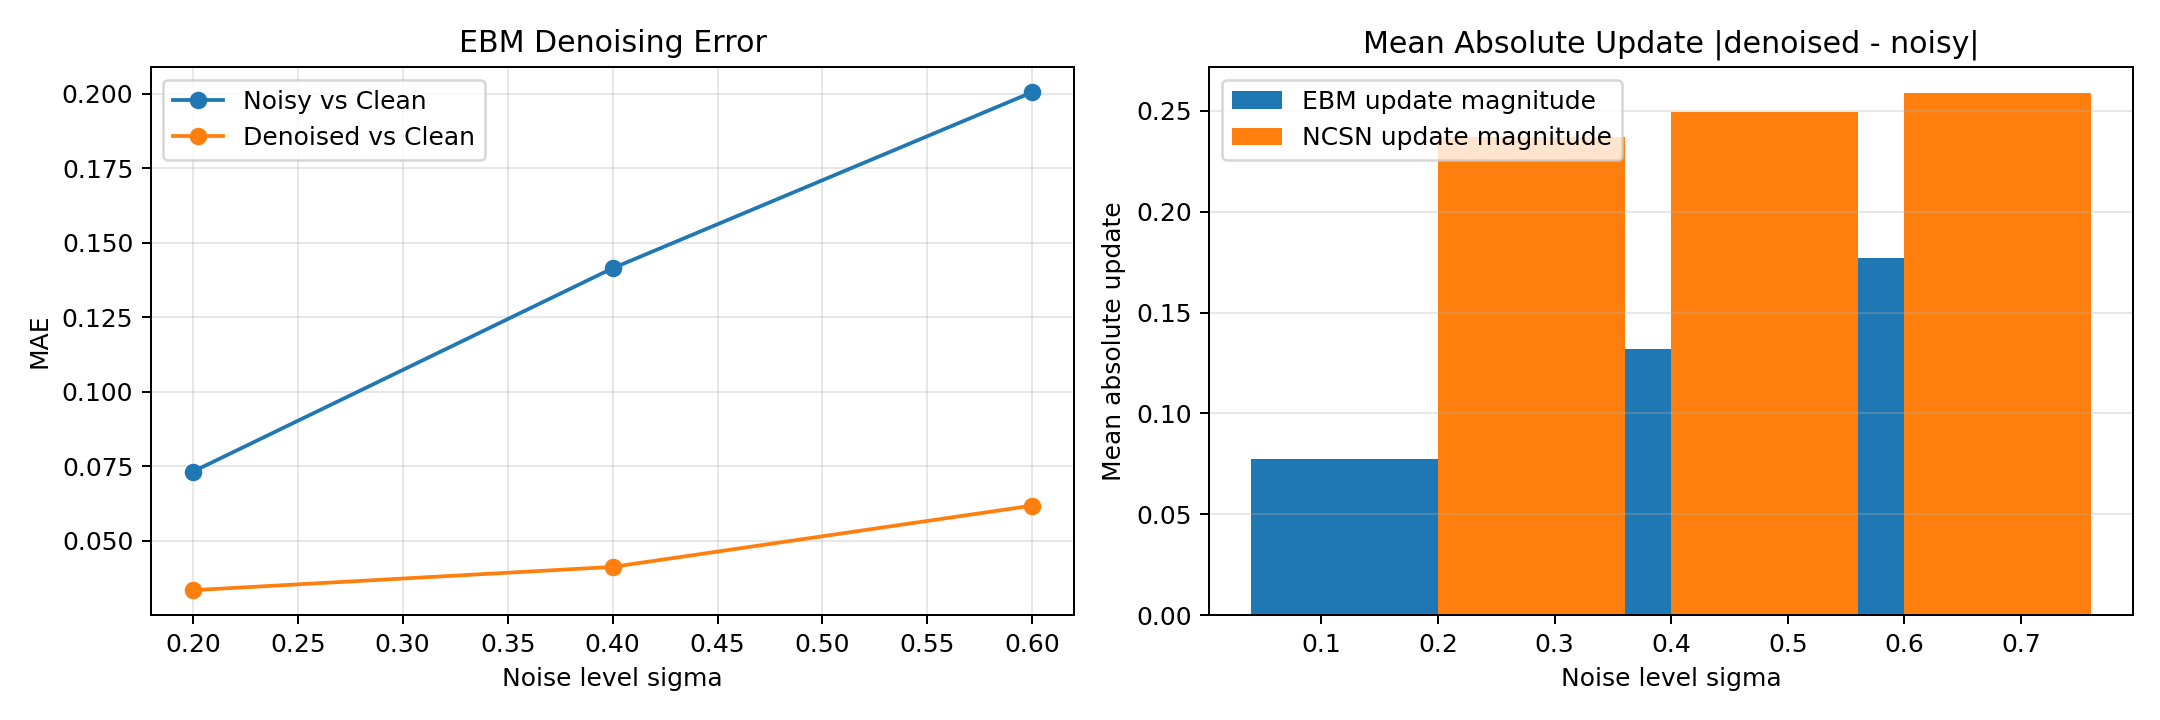
\includegraphics[width=0.95\linewidth]{../images/report/denoise_metrics.png}
    \caption{Supplementary denoising diagnostics derived from archived result
    grids. Left: EBM MAE to clean images before/after denoising. Right:
    mean absolute update magnitude for EBM and NCSN.}
    \label{fig:denoise-metrics}
\end{figure}

\paragraph{Interpretation notes.}
These diagnostics are intended as sanity checks rather than benchmark
metrics. For EBM, clean/noisy/denoised triplets are available and enable
direct MAE-to-clean comparisons. For NCSN, archived outputs include noisy and
denoised grids but not the matching clean grid in the same directory; hence we
report transformation magnitude and Laplacian-variance behavior instead of
clean-target MAE.

\begin{table}[H]
\centering
\caption{EBM denoising diagnostics from archived grids.}
\label{tab:ebm-denoise-metrics}
\begin{tabular}{@{}ccccc@{}}
\toprule
\textbf{$\sigma$} & \textbf{MAE(Noisy,Clean)} & \textbf{MAE(Denoised,Clean)} &
\textbf{MAE Gain} & \textbf{Mean Abs Update} \\
\midrule
0.2 & 0.0732 & 0.0334 & 0.0398 & 0.0773 \\
0.4 & 0.1414 & 0.0412 & 0.1002 & 0.1321 \\
0.6 & 0.2005 & 0.0618 & 0.1387 & 0.1769 \\
\bottomrule
\end{tabular}
\end{table}

\begin{table}[H]
\centering
\caption{NCSN denoising diagnostics from archived grids.}
\label{tab:ncsn-denoise-metrics}
\begin{tabular}{@{}cccc@{}}
\toprule
\textbf{$\sigma$} & \textbf{Mean Abs Update} & \textbf{Laplacian Var Ratio} &
\textbf{Comment} \\
\midrule
0.2 & 0.2368 & 3.1711 & Strong structural sharpening from noisy input. \\
0.4 & 0.2493 & 1.7111 & Moderate sharpening while preserving digit topology. \\
0.6 & 0.2587 & 0.9660 & Heavy correction with near-equal high-frequency energy. \\
\bottomrule
\end{tabular}
\end{table}

\paragraph{Key takeaway.}
For EBM, the MAE gain increases with noise level, indicating that Langevin
refinement remains beneficial even under heavy corruption, although absolute
error still grows as expected. For NCSN, the model applies consistently large
updates across all noise levels, reflecting aggressive correction behavior of
the annealed sampler.

\subsection{Validation and Acceptance Criteria}

Before finalizing the report, we require all checks below to pass:
\begin{itemize}[leftmargin=*]
  \item \textbf{Code import and syntax checks pass:} core scripts compile and
  import without runtime import errors.
  \item \textbf{Checkpoint compatibility holds:} inference can load archived
  EBM/NCSN checkpoints without shape mismatches.
  \item \textbf{Figure integration is complete:} no placeholder figure blocks
  remain in Parts 4 and 7.
  \item \textbf{LaTeX build succeeds:} \texttt{report/main.tex} compiles
  cleanly with \texttt{pdflatex} (two runs for references).
  \item \textbf{Visual inspection passes:} rendered PDF pages show embedded
  figures, correct captions, and no broken glyphs or artifact tokens.
\end{itemize}

\subsection{Final Submission Checklist}

To reduce last-minute errors, the final delivery should include:
\begin{itemize}[leftmargin=*]
  \item Executable Python code under \texttt{codes/} with fixed training and
  inference pipelines for EBM and NCSN.
  \item Report source files under \texttt{report/} and final PDF
  \texttt{report/main.pdf}.
  \item Report-ready figures under \texttt{images/report/}.
  \item A reproducibility script/command path
  (\texttt{codes/generate\_report\_assets.py}) for deterministic figure
  assembly from archived outputs.
  \item Submission packaging using the course naming convention with both code
  and report included.
\end{itemize}

\subsection{Conclusions}

This report provided a comprehensive exploration of energy–based and
score–based generative models on the MNIST dataset.  We derived the
theoretical foundations of EBMs, including the maximum–likelihood
gradient and the challenges of sampling from unnormalised densities.
Contrastive divergence and Langevin dynamics were used to train and
sample from a simple convolutional EBM.  We then introduced score–based
models, explaining how denoising score matching avoids the divergence
term and how multi–scale noise perturbation and annealed Langevin
dynamics enable high–quality sampling.  The noise–conditional score
network was implemented using a U–Net architecture with FiLM
conditioning, and both unconditional and conditional versions were
trained.

Empirically, NCSNs outperformed EBMs in terms of sample sharpness,
denoising ability and ease of conditioning.  EBMs, while flexible in
defining energy functions, suffered from blurriness and required careful
hyperparameter tuning.  The multi–scale training of NCSNs proved
effective at capturing both global and local structures, and the ALD
sampler produced clean digits with relatively few steps.

In summary, score–based models constitute a powerful alternative to
traditional energy–based methods for generative modeling.  They
sidestep the normalisation problem, leverage multi–scale training to
learn rich gradient fields, and produce high–quality samples via
stochastic sampling.  Nonetheless, both paradigms contribute valuable
insights: EBMs offer a principled view of probability densities and
provide a direct measure of compatibility, while score–based models
unlock efficient training and sampling.  Future research will likely
continue to integrate these perspectives, pushing the boundaries of
generative modeling across modalities and applications.
